\section{Hadoop Core}
Der Kern von Hadoop (Hadoop Core) besteht seit Hadoop 2.x aus vier Modulen, welche im offiziellen Download zusammengefasst sind\cite{noauthor_apache_nodate}:
\begin{itemize}
    \item Hadoop Distributed File System (HDFS™): Hadoops verteiltes Dateisystem
    \item Hadoop MapReduce: Hadoops Parallel Processing Engine für große Datenmengen
    \item Hadoop YARN: Ein Framework für Job Scheduling und Ressourcenverwaltung im Cluster
    \item Hadoop Common: Unterstützende Programme für die anderen Hadoop-Module
\end{itemize}
Diese Komponenten bringen alles mit, was man zur verteilten Verarbeitung und Speicherung großer Datenmengen benötigt. 

\subsection{HDFS}
\label{chap:fund sec:core sub:hdfs}
Das HDFS ist ein Dateisystem, welches dem Anwender eine Abstraktionsschicht über verteilt gespeicherte Daten bietet. Das HDFS ist für den Betrieb auf Clustern aus sogenannter \textit{Commodity Hardware} konzipiert. Commodity Hardware ist günstige, leicht zu ersetzende Hardware. Bei Commodity-Hardware-Clustern wird nicht etwa versucht, Ausfälle einzelner Nodes durch den Einsatz von besonders ausfallsicherer (und somit teurer) Hardware zu verhindern. Fällt ein Node aus, was in einem Cluster von hunderten Maschinen kein Sonderfall ist, übernimmt ein anderer Node dessen Arbeit, ohne dass dadurch die Verfügbarkeit des Clusters beeinträchtigt wird. Das HDFS setzt dafür auf die Konzepte von Blöcken, Replikation und Redundanz.\cite{white_hadoop_2015}  
\par
Ein vollwertiger Hadoop Cluster (Hadoop im \textit{fully-distributed Mode}) besteht aus mindestens einem Master, dem \textbf{NameNode}, und einem oder mehr Workern, den \textbf{DataNodes} (\textit{vgl. Abb. }\ref{fig:hdfs}). Um Dateien im HDFS zu speichern, teilt ein \textit{Client}-Prozess die Dateien in Blöcke von standardmäßig 128MB auf und kontaktiert den NameNode. Der NameNode hat einen Überblick über den verfügbaren Speicherplatz aller DataNodes und designiert manche davon, um einige der Blöcke aufzunehmen. Der NameNode achtet außerdem darauf, dass jeder einzelne Block repliziert und auf unterschiedlichen DataNodes gespeichert wird. Standardmäßig verteilt Hadoop drei Kopien eines jeden Blocks im Cluster. Dadurch verbraucht man zwar drei mal so viel Speicher wie bei herkömmlichen, nicht redundanten Dateisystemen, erreicht dafür aber eine sehr hohe Verfügbarkeit. Der Einsatz von Commodity Hardware hält trotz des erhöhten Speicherbedarfs die Kosten niedrig.\cite{white_hadoop_2015}     
\par
Die DataNodes senden in regelmäßigen Abständen sogenannte \textit{Block Reports} an den NameNode. Dieser gleicht die Block Reports mit dem Soll-Zustand des Dateisystems ab. Ist zum Beispiel in einem Node eine Festplatte ausgefallen, so sind manche Blöcke unterrepliziert. Der NameNode veranlasst DataNodes, die Kopien der betroffenen Blöcke besitzen dazu, diese an andere DataNodes zu senden, bis der Soll-Zustand des Clusters wieder hergestellt ist.

\begin{figure}[ht]
    \centering
    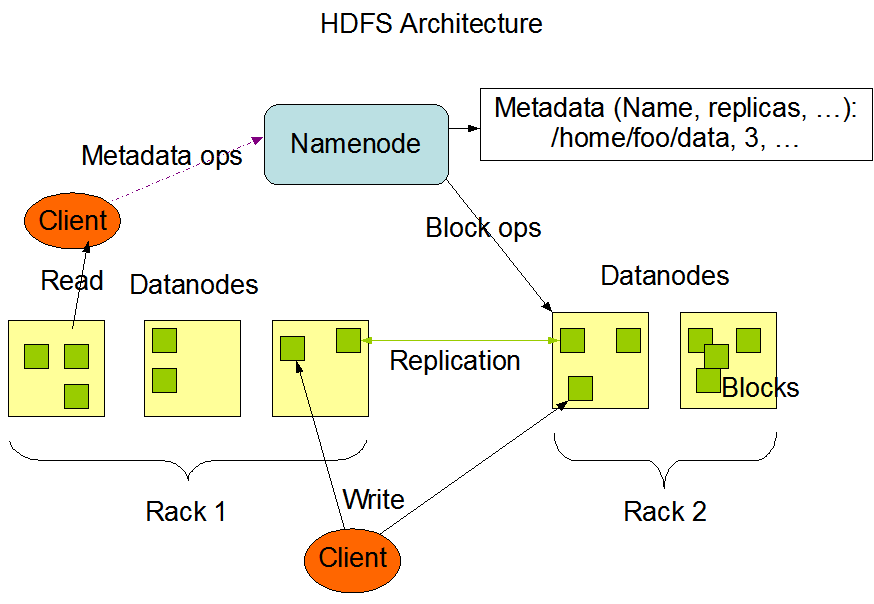
\includegraphics[width=\textwidth]{hdfsarchitecture}
    \caption[Architektur des HDFS]{Architektur des HDFS\parencite{noauthor_apache_nodate-1}}
    \label{fig:hdfs}
\end{figure}

\subsection{YARN}
In Version 1.x von Hadoop war MapReduce sowohl für die Verarbeitung der Daten, als auch für die Ressourcenzuteilung im Cluster zuständig. Das bedeutete, dass man zwingend MapReduce-Applikationen nutzen musste, um die im Hadoop Cluster gespeicherten Daten auszuwerten. MapReduce hat Einschränkungen und Eigenheiten, auf die in Abschnitt \ref{chap:fund sec:core sub:mapred} eingegangen wird. Weiterhin war die Ressourcenverwaltung damit ein mögliches Bottleneck, da sie bei mehreren parallel laufenden Jobs auf einem Node um Rechenzeit mit der Datenverarbeitung konkurrieren musste.\cite{freiknecht_big_2018}
\par
Die größte Änderung in Hadoop 2.x war dann die Ausgliederung der Ressourcenverwaltung aus MapReduce und die Einführung einer dedizierten Ressourcenverwaltungsanwendung - \textbf{YARN} - \textit{Yet Another Ressource Negotiator}. YARN teilt eingehenden Jobs Cluster-Ressourcen zu und startet fehlgeschlagene Jobs gegebenenfalls neu.\cite{freiknecht_big_2018} Ähnlich wie das HDFS bringt YARN eine Reihe von Prozessen mit sich, die Master- und Worker-Rollen einnehmen. Auf \textit{einem} Node im Cluster, nämlich dem vom HDFS designierten NameNode, läuft der \textbf{Resource Manager}. Dieser unterteilt sich wiederum in \textbf{Application Manager} und \textit{Scheduler}. Auf allen DataNodes laufen jeweils ein \textbf{Node Manager} und ein \textbf{Application Master}. 
\par

\subsection{Setup}
\subsubsection*{Single Node Setup}
Defaulteinstellung des Hadoop Downloads
Installation auf der einen beteiligten Maschine
Start eines Single Node Clusters lokal
Erste Übung zum Umgang mit dem HDFS
\subsubsection*{Fully-distributed Cluster}
Installation von Hadoop auf allen beteiligten Maschinen
Einrichtung von passwordless ssh auf allen Maschinen
Evtl. Anpassung der /etc/hosts auf allen Maschinen
Editieren der ganzen Konfigurationsdateien (XML) und kopieren der gleichen Dateien auf alle beteiligten Maschinen
Editieren der Worker Datei auf dem NameNode
NameNode (HDFS) formatieren
Ausführen der Skripte auf dem NameNode

\subsubsection*{Hadoop in der Cloud}
Google Dataproc, Azure HDInsights
Oftmals eigenes Dateisystem, fully managed
Grafische Oberfläche zum Submitten von Jobs, etc.

\subsection{MapReduce}
\label{chap:fund sec:core sub:mapred}
MapReduce Workflow: Erstellung eines MapReduce Jobs, Kopieren auf den Name Node und Ausführung
